\documentclass[12pt,a4paper,titlepage]{article}
\usepackage[utf8]{inputenc}
\usepackage{amsmath}
\usepackage{amsfonts}
\usepackage{amssymb}
\usepackage{supertabular}
\usepackage{tabularx}
\usepackage{ltablex}
\usepackage{graphicx}
\usepackage{pdfpages}
\usepackage[left=1in,right=1in,top=1in,bottom=1in]{geometry}
\parskip=0pt
\title{ 
\center
\includegraphics[width=\linewidth]{UIGraphic}\\
		\center\textbf{\Large{System and Software Design Description(SSDD):}\\
		\large{Incorporating Architectural Views and Detailed Design Criteria\\
		For\\
		\large{Swords and Sorcery(S\&S)}}\\
		Version 1.0}}
\author{Prepared by:\\University of Idaho Computer Science 383 Class, Spring 2014\\
\bigskip\\
Prepared for:\\
Dr. Clinton Jeffery\\} 
\date{\today} 
\begin{document}
\maketitle
\pagebreak
\setcounter{tocdepth}{3}
\renewcommand\contentsname{\center{Swords and Sorcery Design\\Table of Contents}}
\tableofcontents
\pagebreak

\section{Introduction}
This is the System and Software Design Document for the computer adaptation of the Swords and Sorcery board game. This is one of five documents that describe the computer adaptation of the Swords and Sorcery board game. The computer adaptation was developed by the Software Engineering class at the University of Idaho in Spring 2014.
\subsection{Document Purpose, Context, and Intended Audience}
\subsubsection{Document Purpose}
The purpose of this document is to describe the system and software design of Swords and Sorcery. This includes diagrams developed to guide design of S\&S, component descriptions, view descriptions, and requirements traceability.
\subsubsection{Document Context}
This document is written as part of a larger document that describes the Swords and Sorcery project developed by the CS383 students at University of Idaho, in Spring 2014. This document only describes the system and software design of the project, which is only a subset of the project.
\subsubsection{Intended Audience}
This document is intended to be read by Dr. Clinton Jeffery and members of the class, as well as any interested members of the University of Idaho Computer Science department. This document is not intended to be distributed publicly in any way.
\subsection{Software Purpose, Context, and Intended Audience}
\subsubsection{System and Software Purpose}
The purpose of the Swords and Sorcery system and software is to provide a computer adaptation of the complex board game of the same name. The system is designed to provide multiplayer functionality over the internet, and to simplify the complex rules of the original Swords and Sorcery.
\subsubsection{System and Software Context}
The context of this project is, again, restrained to the classroom, as it is an educational project, not intended for distribution. However, the source code for the project, as well as many resources, are available publicly on github.com. 
\subsubsection{Intended Users of System and Software}
The intended users of the Swords and Sorcery system are the developers (students of CS383) and any outgoing, motivated individuals who find the S\&S source on www.github.com. Also included in intended users is the class instructor, Dr. Clinton Jeffery. 
\subsection{Definitions, Acronyms, and Abbreviations}
\small{
\begin{center}
\keepXColumns
\noindent\begin{tabularx}{\linewidth}{|p{1.5in}|X|}\hline
\textbf{Term} & \textbf{Definition}\\
\hline
AD & Architectural Description: \"A collection of products to document an architecture.\"\space ISO/IEC 42010:2007\\
\hline
Alpha Test & Limited release(s) to selected, outside testers.\\
\hline
Architectural View & \"A representation of a whole system from the perspective of a related set of concerns.\"\space ISO/IEC 42010:2007\\
\hline
Architecture & \"The fundamental organization of a system embodied in its components, their relationships to each other, and to the environment, and the principles guiding its design and evolution.\"\space ISO/IEC 42010:2007\\
\hline
Army Unit & An instance of the class ArmyUnit, which is a subclass of MovableUnit.\\
\hline
Beta Test & Limited release(s) to cooperating customers wanting early access to developing systems.\\
\hline
Client & The process the user directly interacts with, containing, among other things, the GUI.\\
\hline
Design Entity & \"An element (component) of a design that is structurally and functionally distinct from other elements and that is separately named and referenced.\"\space IEEE STD 1016-1998\\
\hline
Design View & \"A subset of design entity attribute information that is specifically suited to the needs of a software project activity.\"\space IEEE STD 1016-1998\\
\hline
Edge & The edge between two hexes. Edges can include roads, walls, streams, etc. and can effect movement or combat\\
\hline
GUI & Graphical User Interface - What the user sees and interacts with - also called the HUD.\\
\hline
Hexagon & A hexagon shaped location on the game or diplomacy map that can contain things like units, edges, or terrain. Or the mathematical hexagon shape.\\
\hline
HexID & A unique hex identification string.\\
\hline
HUD & Heads Up Display - What the user sees, with respect to interface - also called the GUI.\\
\hline
IP & Internet Protocol - Typically refers to an IP Address.\\
\hline
PlayerID & An integer representing one of the factions described in this scenario.\\
\hline
S\&S & Swords and Sorcery\\
\hline
Server & The (single) process that a client connects and sends messages to. \\
\hline
SSDD & System and Software Design Document\\
\hline
SSRS & System and Software Requirements Specification\\
\hline
System & \"A collection of components organized to accomplish a specific function or set of functions.\"\space ISO/IEC 42010:2007\\
\hline
System Stakeholder & \"An individual, team, or organization (or classes thereof) with interests in, or concerns, relative to, a system.\"\space ISO/IEC 42010:2007\\
\hline
Unit & An instance of a MoveableUnit\\
\hline
\end{tabularx}
\end{center}
}

\subsection{Document References}
\begin{enumerate}
\item CSDS, textit{System and Software Requirements Specification Template}, Version 1.0, July
31, 2008, Center for Secure and Dependable Systems, University of Idaho, Moscow, ID, 83844.

\item ISO/IEC/IEEE, \textit{IEEE Std 1471-2000 Systems and software engineering -- Recommended practice for architectural description of software intensive systems,} First edition 2007-07-15, International Organization for Standardization and International Electrotechnical Commission, (ISO/IEC), Case postale 56, CH-1211 Geneve 20, Switzerland, and The Institute of Electrical and Electronics Engineers, Inc., (IEEE), 445 Hoes Lane, Piscataway, NJ 08854, USA.

\item IEEE, \textit{IEEE Std 1016-1998 Recommended Practice for Software Design Descriptions}, 1998-09-23, The Institute of Electrical and Electronics Engineers, Inc., (IEEE) 445 Hoes Lane, Piscataway, NJ 08854, USA.

\item 3) ISO/IEC/IEEE, \textit{IEEE Std. 15288-2008 Systems and Software Engineering -- System life cycle processes,}Second edition 2008-02-01, International Organization for Standardization and International Electrotechnical Commission, (ISO/IEC), Case postale 56, CH-1211 Geneve 20, Switzerland, and The Institute of Electrical and Electronics Engineers, Inc., (IEEE), 445 Hoes Lane, Piscataway, NJ 08854, USA.

\item ISO/IEC/IEEE, IEEE Std. 12207-2008, \textit{Systems and software engineering -- Software life cycle processes}, Second edition 2008-02-01, International Organization for Standardization and International Electrotechnical Commission, (ISO/IEC), Case postale 56, CH-1211 Geneve 20, Switzerland, and The Institute of Electrical and Electronics Engineers, Inc., (IEEE), 445 Hoes Lane, Piscataway, NJ 08854, USA.
\end{enumerate}

\subsection{Overview of Document}
\paragraph{Section 2} of this document describes the concerns and constraints of the system and software, with respect to environmental constraints, system requirement constraints, and user characteristic constraints. Section 2 also describes stakeholder concerns.
\paragraph{Section 3} of this document describes the System and Software architecture of Swords and Sorcery, from different points of view, namely the user's point of view and the developer's point of view.
\paragraph{Section 4} of this document describes the finer details of the software design, listing software and system components that are crucial to the operation of the Swords and Sorcery game. 
\paragraph{Section 5} of this document describes the requirements traceability of the Swords and Sorcery project, highlighting how our original project requirements have been met, modified, and implemented.
\subsection{Document Restrictions}
This document is for LIMITED USE ONLY to UI CS personnel working on the project.
\section{Constraints and Concerns}

\subsection{Constraints}
Swords and Sorcery requires the Java Runtime Environment 8 to run. S\&S also requires the JDK 8.0 and Netbeans 8.0 or better to develop, or a proficiency with ANT, which is the directory structure the project uses, as a result of being developed in Netbeans. The game will run on Windows, Mac, and Linux, provided those systems have the mentioned software packages (JRE to play, JDK/Netbeans to develop). To play the game, a network connection is required, as well as the IP Address of the game server. As S\&S is a multiplayer game, one client is required for each player. Typically, this should be done using multiple computers, however, multiple clients can be run on the same computer.

\subsection{Stakeholder Concerns}
There are no financial stakeholders, however, Dr. Clinton Jeffery can be considered a stakeholder, as well as each class member. As a class member, our concerns are providing a quality product, while Dr. Jeffery's concerns may include using good design principles, as this is a Software Engineering course. 
Other concerns include design requirements such as portability, 

\section{System and Software Architecture}
\subsection{Developer's Architectural View}
\subsubsection{Developer's View Identification}
There are multiple developer views within the scope of the S\&S project for CS383. The views represent each subteam, and there are three subteams - HUD Team, Rules Team, and Networking Team. The descriptions of each sub-view follow, as well as an overview diagram.
\paragraph{HUD Team View} The HUD Team view includes all software design related to the HUD/GUI and handles how the user(s) interact with the S\&S game rules and networking. 
\paragraph{Rules Team View} The Rules Team view includes all software implementations of the S\&S rule set, some of which overlaps with other views. Typically, Rules Team is in charge of implementing internal logic and data structures.
\paragraph{Networking Team View} The Networking Team view includes all network communication related to the S\&S game. This includes the client/server model, the communication protocols, the server setup and more.
\subsubsection{Developer's View Representation and Description}
\paragraph{Architectural Overview}
The following class diagram is inaccurate with respect to the project as it currently stands. The inaccuracies are the Chart class, which does not exist, and we discovered is unnecessary, as well as the alliance and player classes, which were never created. The alliance class was never created because we didn't make it that far with the project, and the player class was replaced with flags and variables, as a class was determined to be unneeded. Also, the diagram lacks references and design information relating the classes to the HUD and Networking components of S\&S.
\begin{center}
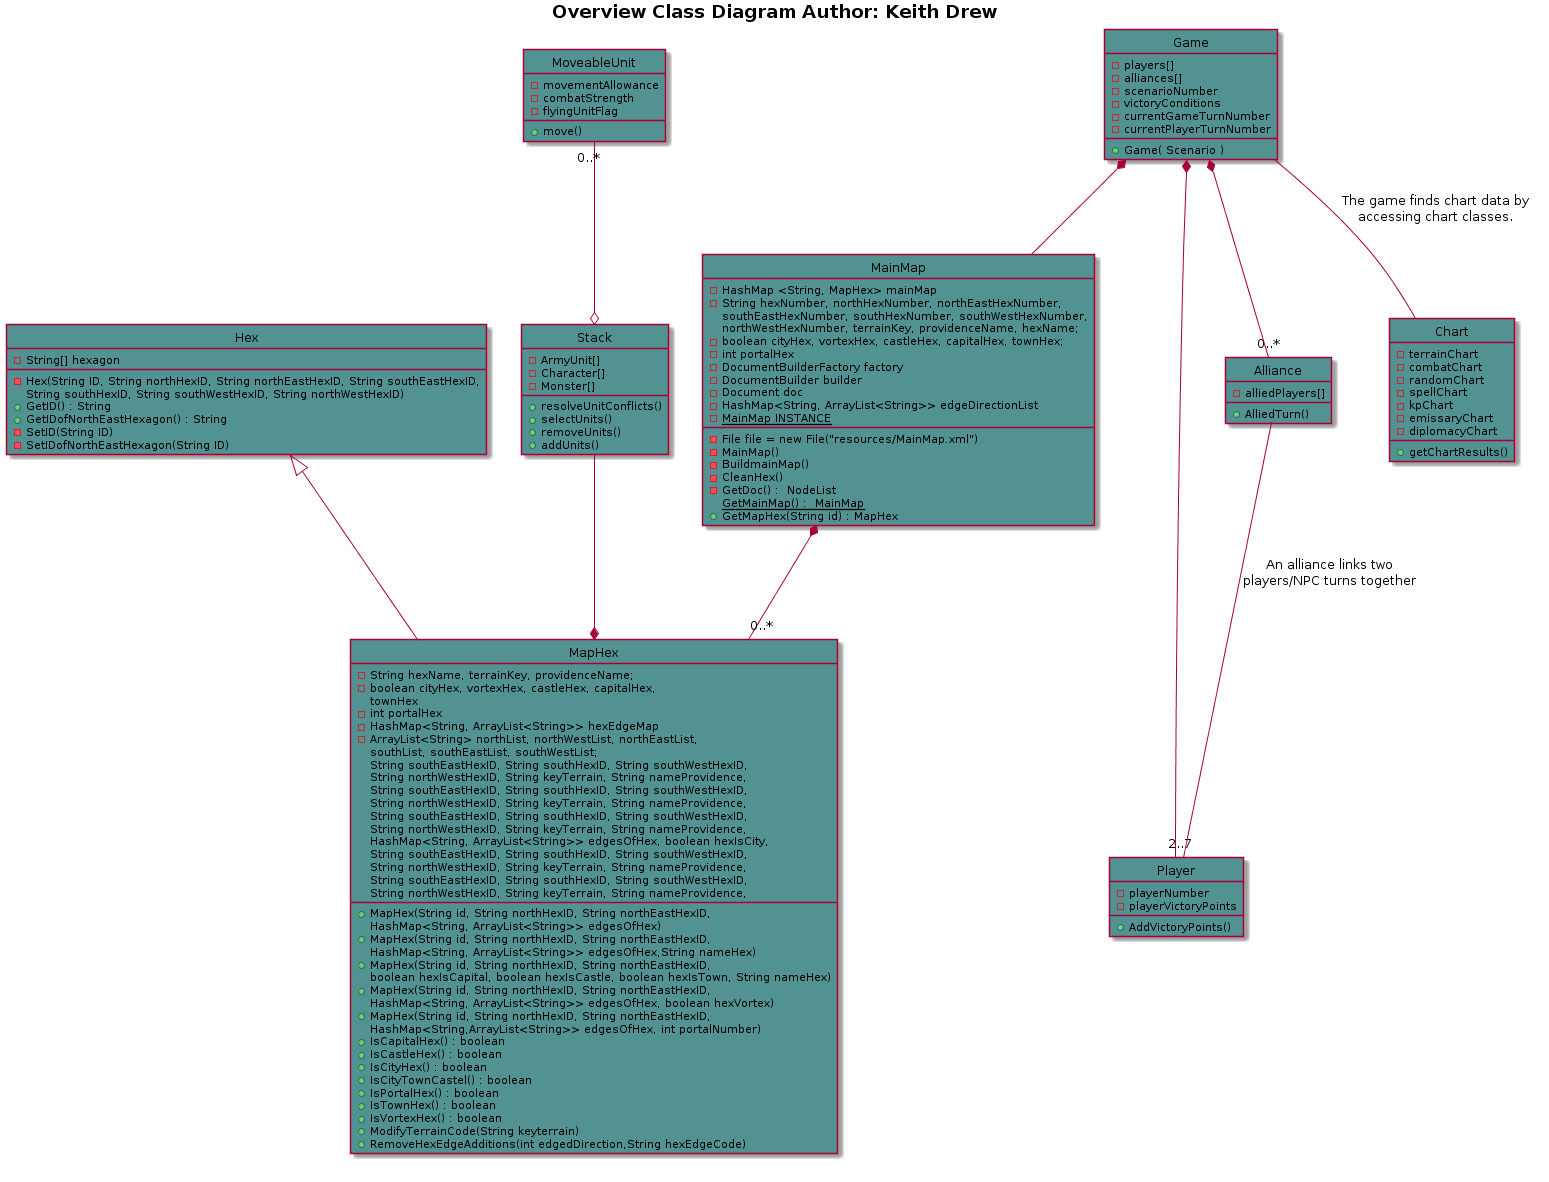
\includegraphics[width=\linewidth]{overview.png}
\end{center}
\paragraph{HUD Team View Representation and Description}
The HUD team view includes rules that affect the HUD (movement, hex painting, terrain, etc.) and the actual HUD itself, containing a view of the map, the minimap, character/unit descriptions, the solar display, the main menu, and hosting interactions between the game instance and the user. The HUD team also designed several data structures include the UnitPool and MainMap, for displaying the units and map in the HUD. Following is a collaboration diagram that shows a rough idea of the design from the HUD Team view.
\begin{center}
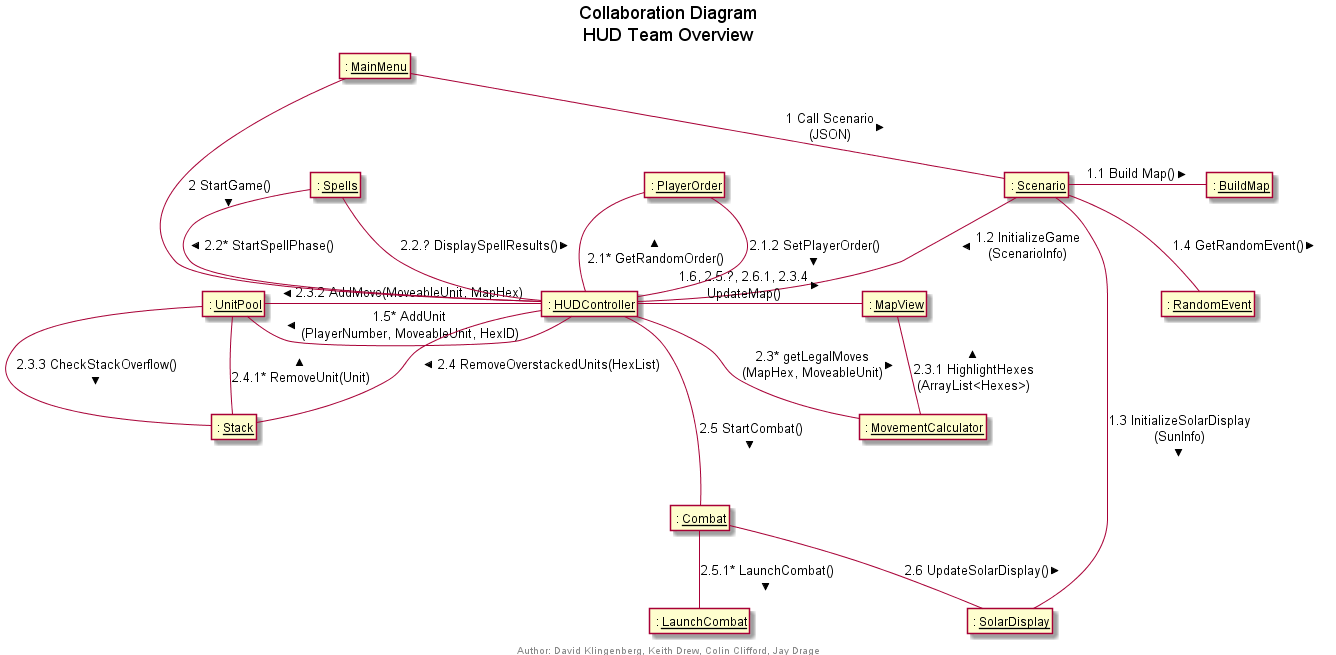
\includegraphics[width=\linewidth]{HUDTeamCollab.png}
\end{center}
\paragraph{Rules Team View Representation and Description}
The rules team view covers the implementation of the rules from the actual boardgame, S\&S. This includes things like combat, spell casting, charts implementation, unit implementation and other rules related tasks. The design view for the rules team consists of how those rules interact with each other and the other groups (HUD, Networking).
%\includegraphics[scale=•]{•}
\paragraph{Networking Team View Representation and Description}
The networking team view covers the client/server implementation and design for S\&S. Their overall view of design was a client/server model which hosts communication over the network and message passign for updating the state of a game. 
%\includegraphics[scale=•]{•}

\subsection{User's Architectural View}
\subsubsection{User's View Identification}
The User's view consists of their interactions with the S\&S GUI. This includes starting the client, joining/starting a game lobby, beginning a game, and interacting with the game. Found here are diagrams representing sequence of play and mouse/key button presses.
\subsubsection{User's View Representation and Description}
\begin{center}
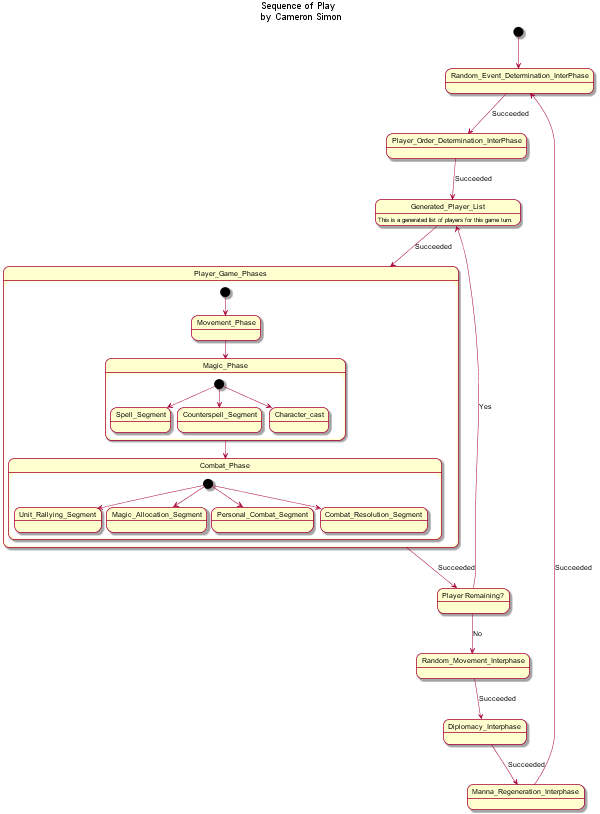
\includegraphics[width=\linewidth]{SequenceOfPlay.png}
\end{center}	
\pagebreak
\begin{center}
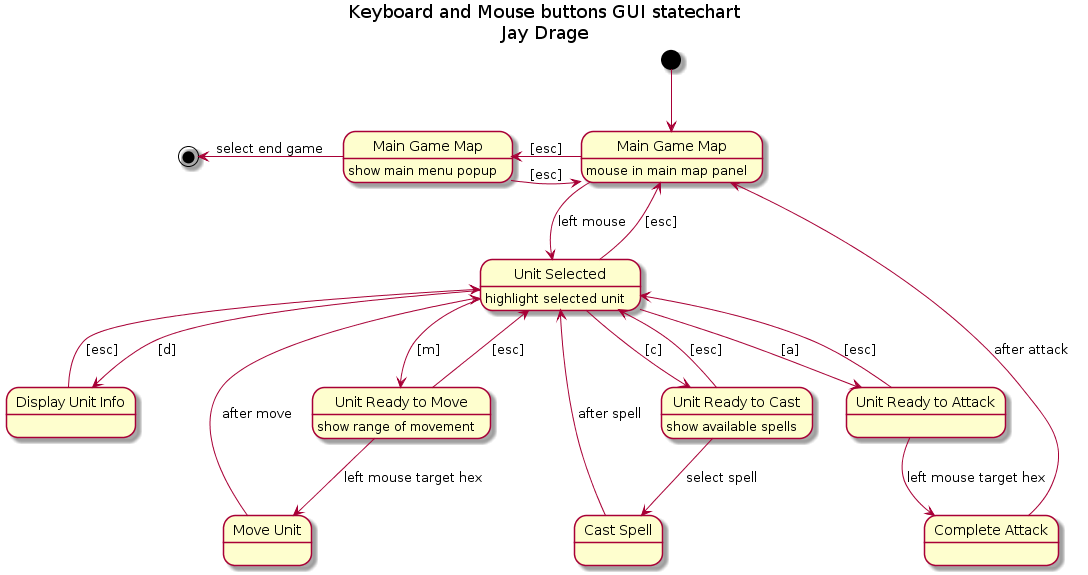
\includegraphics[width=\linewidth]{KeyMouseButtons.png}
\end{center}
\pagebreak

\section{Software Detailed Design}
\subsection{Developer's Viewpoint Detailed Software Design}
This section describes the developers viewpoint with respect to the software design. Included are the UML diagrams developed for the S\&S game, from which we began designing S\&S, as well as the state and collaboration diagrams. Many of the diagrams were developed at different points during the semester, reflected by the discrepancies between the SSRS, this document, and the Implementation document. 
\subsubsection{UML Class Diagrams}
\begin{center}
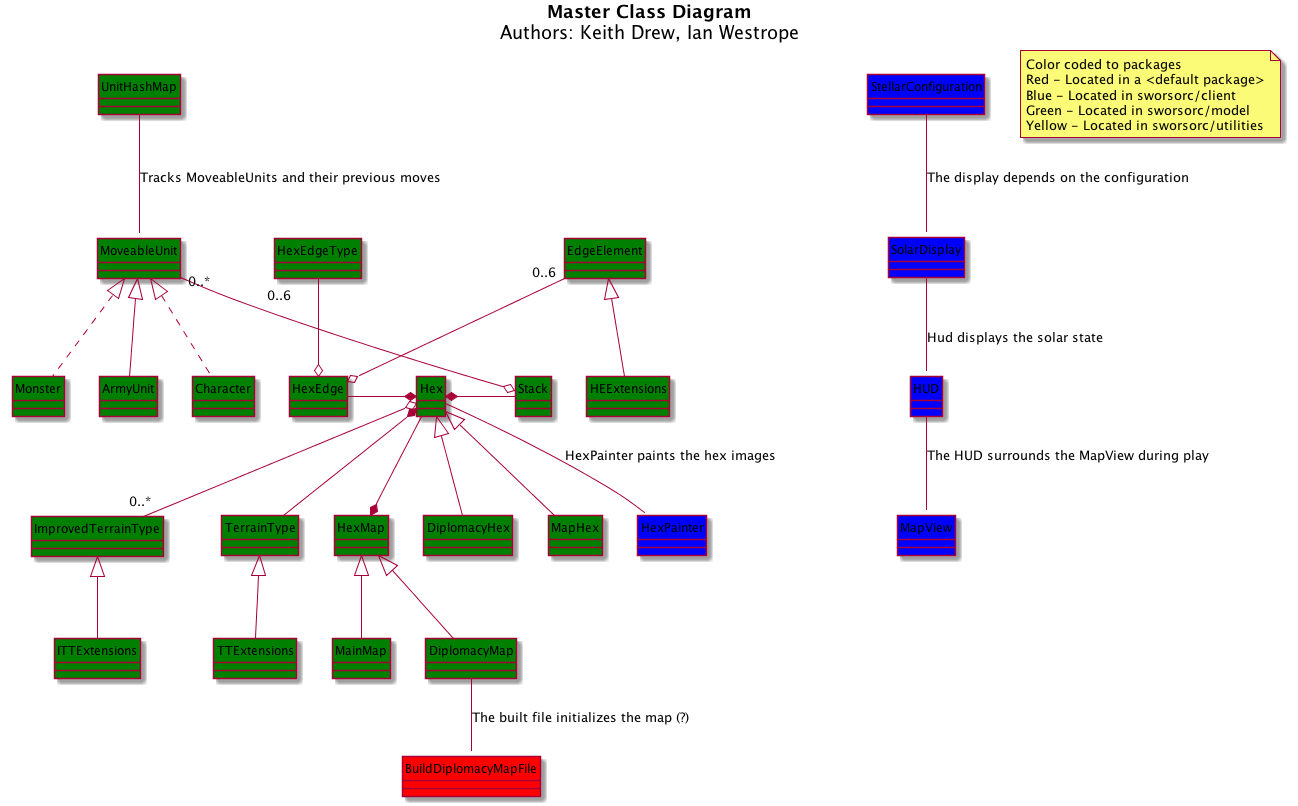
\includegraphics[width=\linewidth]{classDiagram.png}
\end{center}
\begin{center}
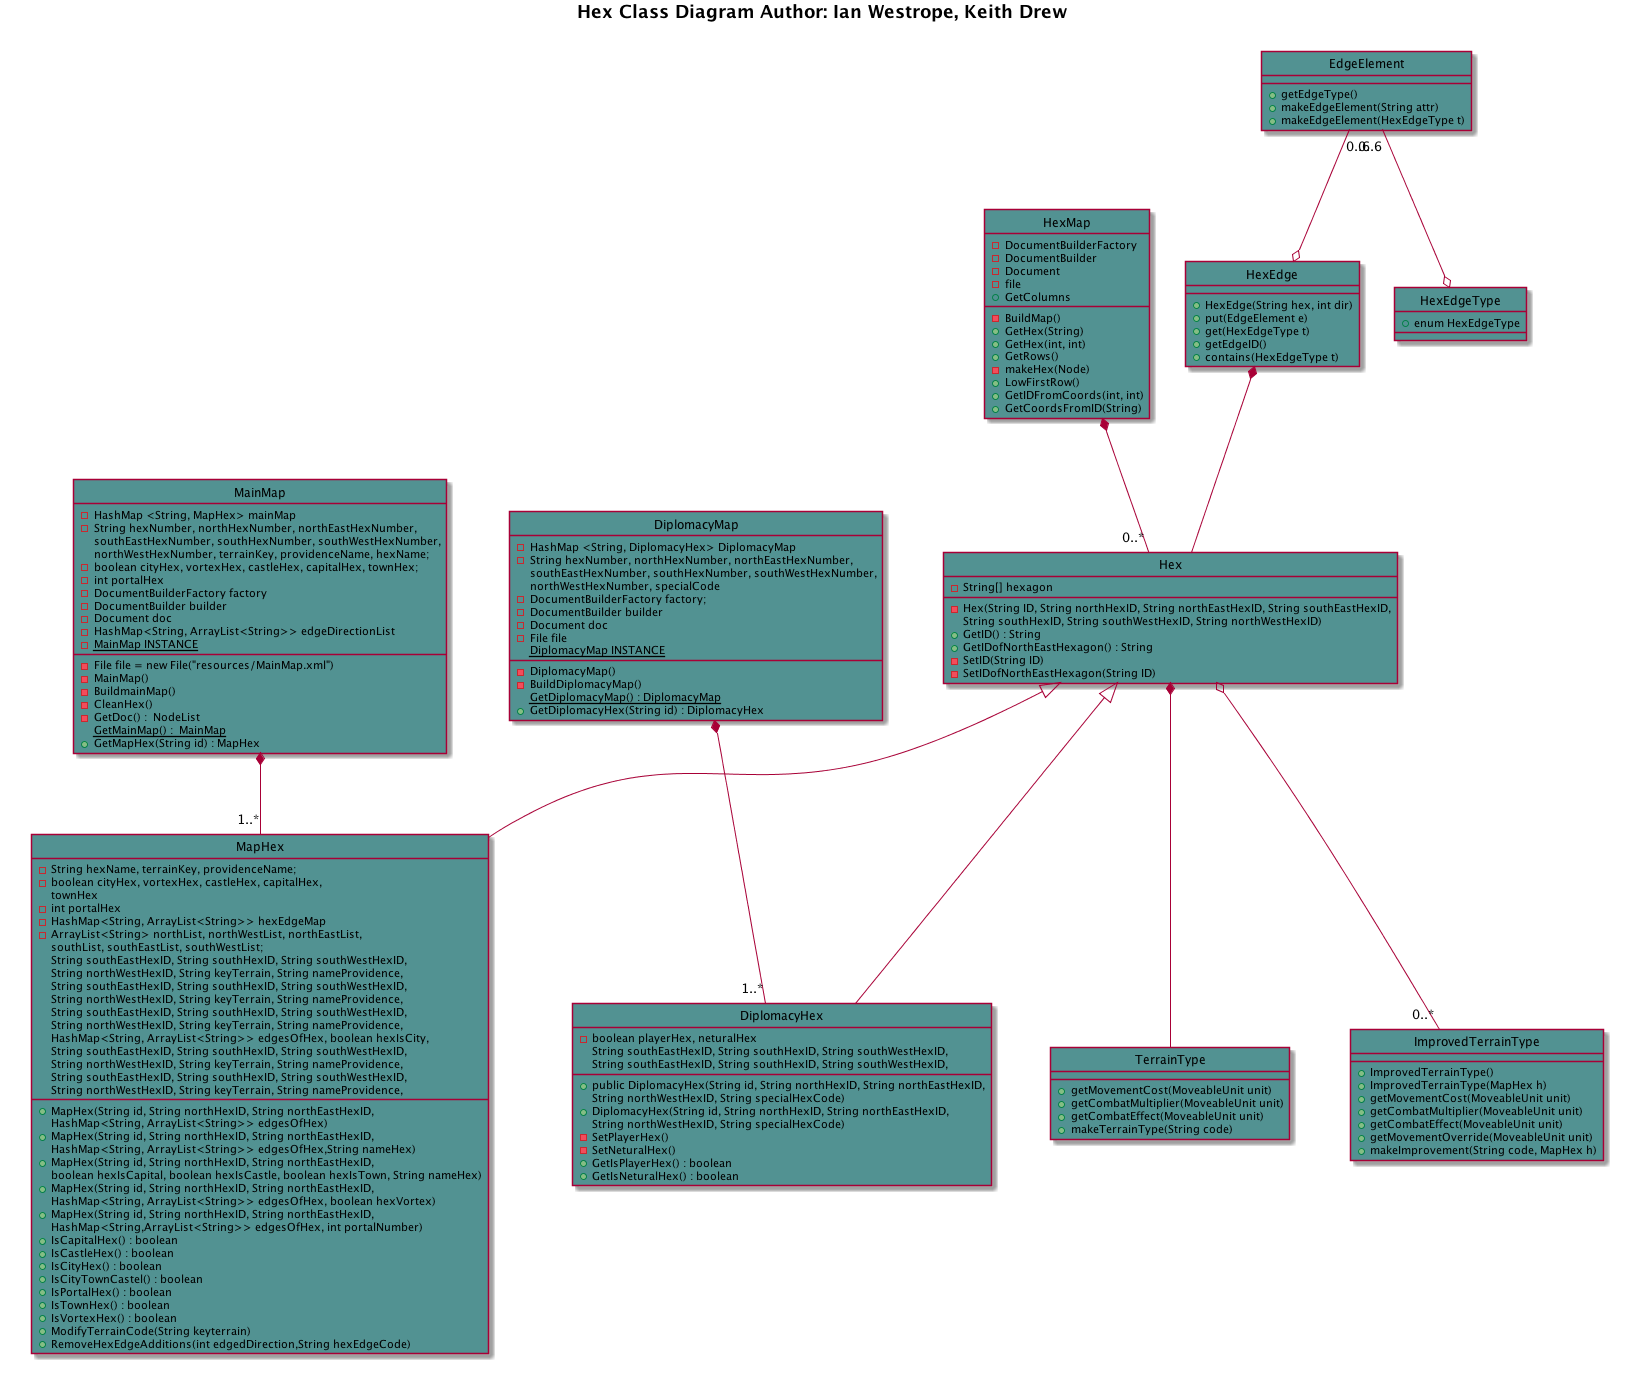
\includegraphics[width=\linewidth]{hex.png}
\end{center}
\begin{center}
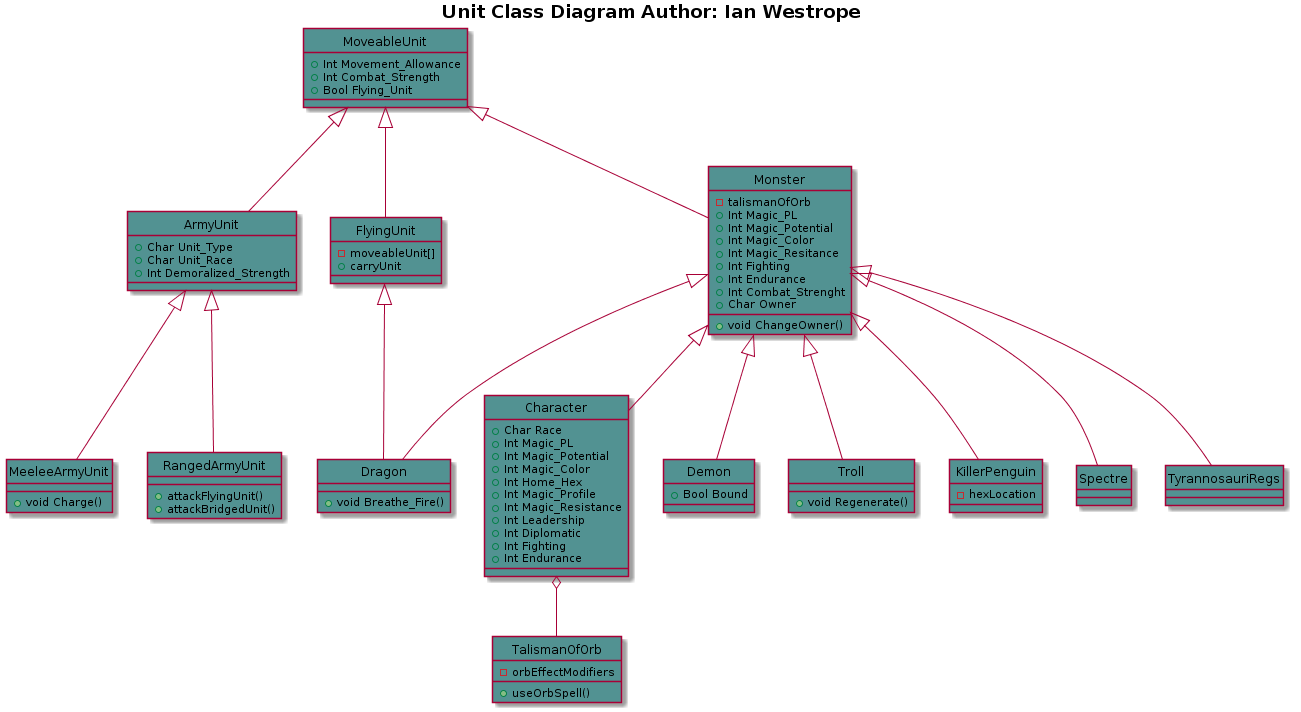
\includegraphics[width=\linewidth]{units.png}
\end{center}
\begin{center}
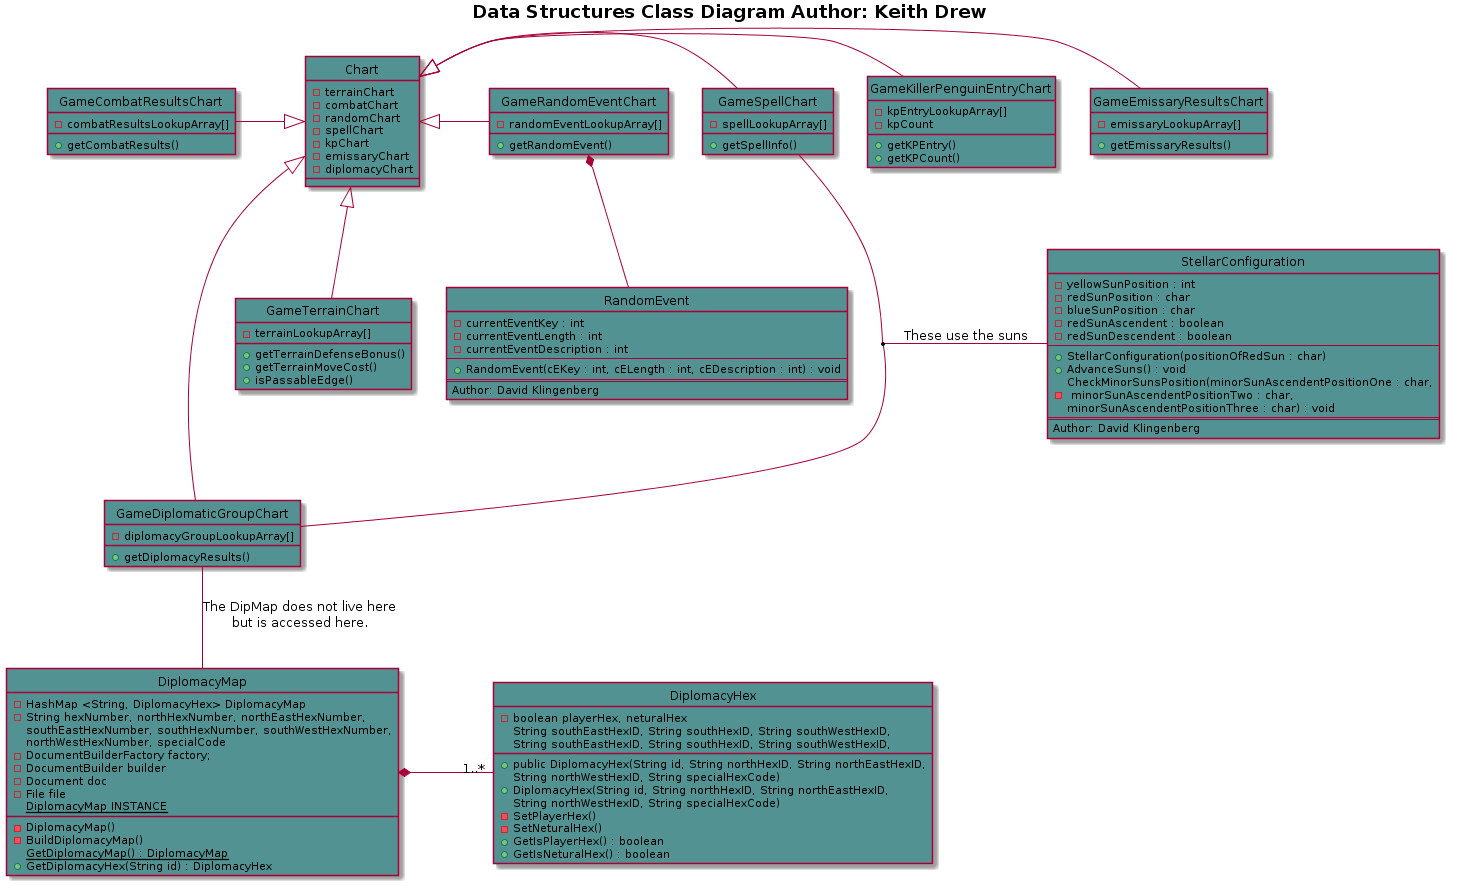
\includegraphics[width=\linewidth]{dataDiagram.png}
\end{center}
\pagebreak
\subsubsection{UML Collaboration Diagrams}
\begin{center}
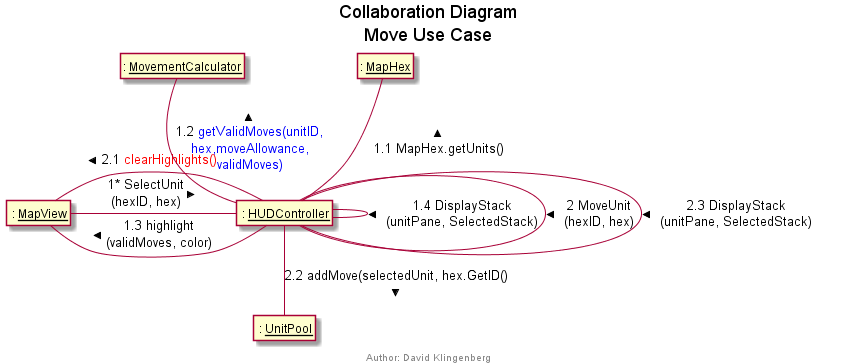
\includegraphics[width=\linewidth]{CollaborationMoveUnit.png}
\end{center}
\pagebreak
\subsubsection{UML State Charts}
\begin{center}
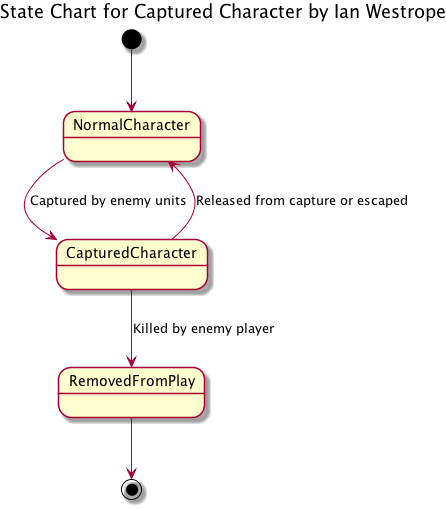
\includegraphics[width=\linewidth]{CharacterCapture}
\end{center}
\begin{center}
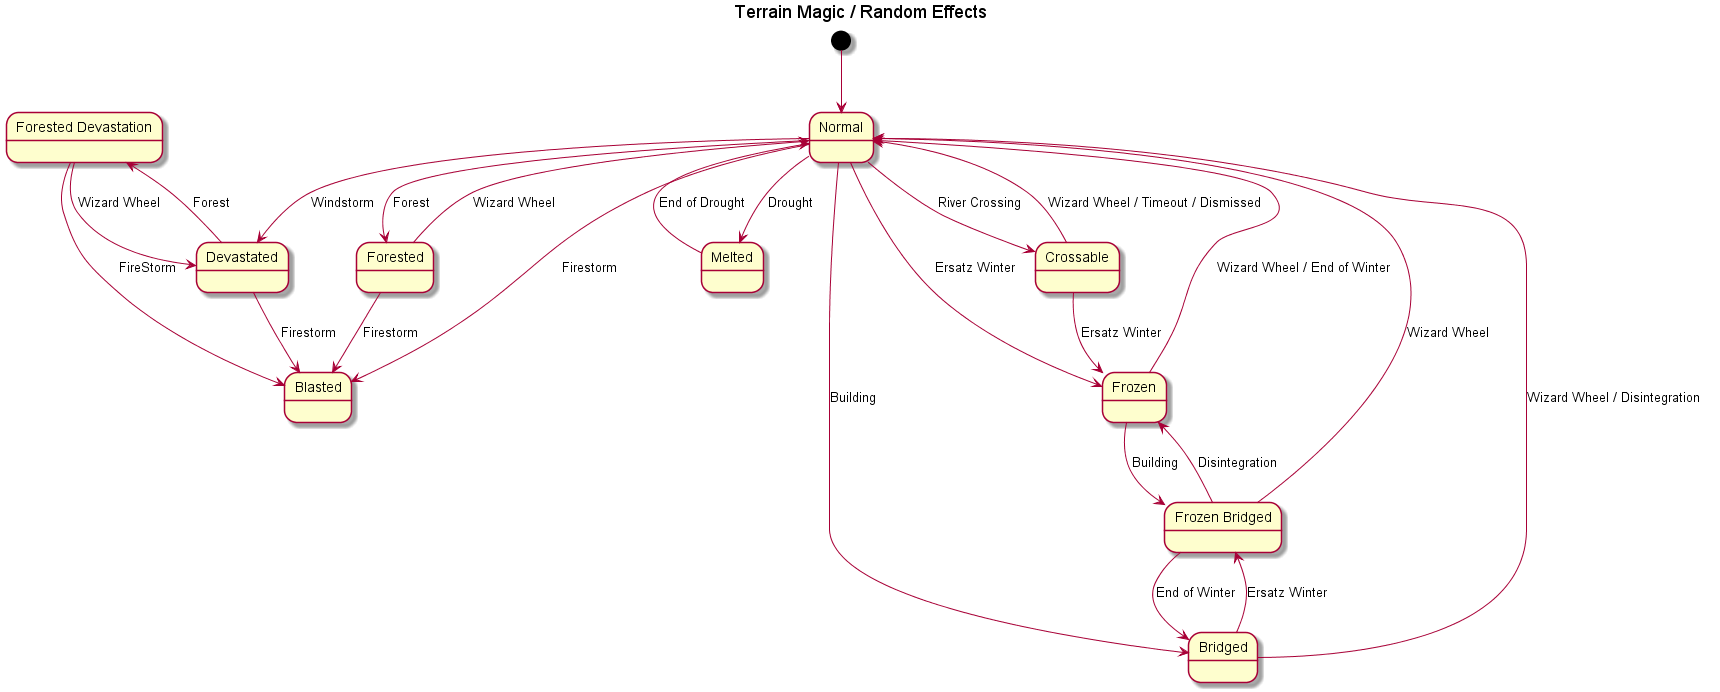
\includegraphics[width=\linewidth]{RandomSpellTerrainEffectsOverview.png}
\end{center}
\begin{center}
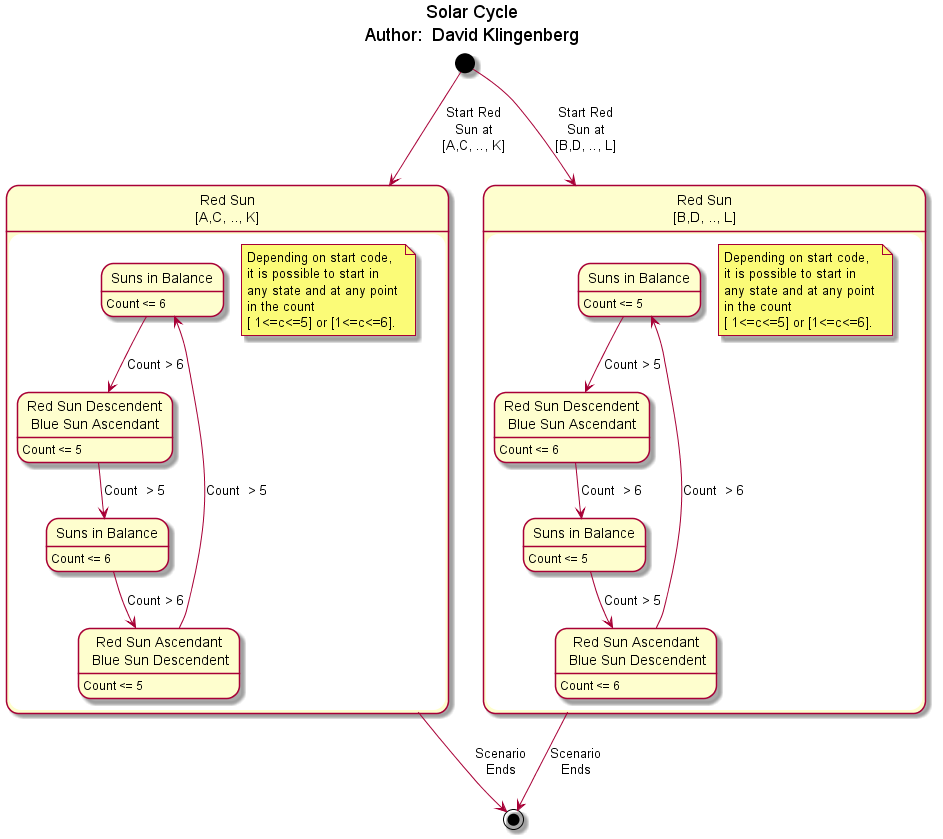
\includegraphics[width=\linewidth]{SolarCycle.png}
\end{center}
\pagebreak
\subsection{Component Dictionary}
\small{
\begin{center}
\keepXColumns
\noindent\begin{tabularx}{\linewidth}{|p{1.5in}|X|X|X|X|}\hline
\textbf{Name} & \textbf{Type/Range} & \textbf{Purpose} & \textbf{Dependencies} & \textbf{Subordinates}\\
\hline
AddMove & UnitPool Method & Move a unit to a new hex & Two array lists: hexList, unitMove & None\\
\hline
AddUnit & UnitPool Method & Add a unit to the sorted tree map & Tree map: pool & None\\
\hline
Army Combat Result Table & Static Method & Determine results of combat lookup & Two ArrayLists: Attackers, Defenders & None\\
\hline
Army Unit & Class & Unit SubClass & Moveable Unit & All individual unit types\\
\hline
Characters & Class & Unit SubClass & Moveable Unit & None\\
\hline
Clear & UnitPool Method & Cleans up the UnitPool for testing purposes. & The entire data structure & None\\
\hline
ClearOverStack & UnitPool Method & Clears an over-stacked array. & Sorted map: overStackMap & None\\
\hline
ClientObject & Class & Represents an open connection to a client from the server. & Tag, Flag, MessagePhoenix & \\
\hline
Conductor & Class & Contains public handler methods for incoming network methods. & Tag, Flag & \\
\hline
EndMovementPhase & UnitPool Method & Prepares the UnitPool for the next move phase. & Sorted map: unitMove & None\\
\hline
Flag & Enum Class & An enumerate constant class providing identifiers for each concrete type of network message. & & \\
\hline
GetAllPlayerUnits & UnitPool Method & Gets all player units. & Tree map: pool & None\\
\hline
GetInstance & UnitPool Method & Gets a Singleton instance of UnitPool. & None & None\\
\hline
GetOverStack & UnitPool Method & Gets hexes in violation of over-stack rule. & Tree map: overStackMap & None\\
\hline
GetPlayerSpecificUnits & UnitPool Method & Get all units by type owned by a player. & Sort map: pool & None\\
\hline
GetSafeTeleport & UnitPool Method & Determine if a unit can safely teleport. & Array list: safeTeleport & None\\
\hline
GetTeleportDestination & UnitPool Method & Get a unit destination portal. & Sorted map: portalNum & None\\
\hline
GetUnit & UnitPool Method & Retrieves a  units. & Sorted map: pool & None\\
\hline
GetUnitHexMove & UnitPool Method & Retrieves all hexes a unit has moved through. & Array list: unitMove & None\\
\hline
GetUnitInHex & UnitPool Method & Retrieves all units in a hex. & Array list: hexList & None\\
\hline
Hexagon Classes & Model & Represents a hexagon & Hex Edge Classes, Terrain Classes, UnitPool & \\
\hline
Hex Edge Classes & Model & Classes to collect and represent elements on hexagon edges & Hex Classes & \\
\hline
HexStack & Class & Ensure compliance with the games stacked rules. & UnitPool & None\\
\hline
HexStacked & Class & Implements rules for stacks. & UnitPool & None\\
\hline
Hexagon Map Classes & Model & Classes to represent a "map" of hexagons, either diplomacy or game. & Hex Classes & \\
\hline
Launch Combat & Static Method & Implement Combat Phase & Moveable Unit, Army Combat Results Table, HUDController, MovementCalculator & None\\
\hline
Lobby & Class & A server-side object that manages a grouping of client connection. & Tag, Flag, MessagePhoenix & \\ 
\hline
MainMenuController & Controller & Define and limit access to main menu & Game.java & \\
\hline
Map Rendering Classes & View & Renders the game map and things on it & MapView, Hexagon Classes, Hex Edge Classes & \\
\hline
MapView & View & A GUI widget to act as a container for the Map Rendering code & Hexagon Classes, Map Rendering Classes & \\
\hline
MessagePhoenix & Utility Class & Used to pack, unpack, send and receive messages over the network & Tag, Flag & \\
\hline
Moveable Unit & Class & Unit SuperClass & None & ArmyUnit, Character, Monster\\
\hline
MovementCalculator & Static Class & Determine Legal Moves & UnitPool, MainMap & Retreat/Move\\
\hline
NetworkClient & Class & Manages network connection for client. & Tag, Flag, MessagePhoenix & Conductor \\
\hline
NetworkServer & Class and Process & The independent server process that clients connect to. & Tag, Flag, MessagePhoenix & ClientObject\\
\hline
OverStackWarning & Static Method & Notifies player of an over-stack condition. & UnitPool & HUDController\\
\hline
RemoveOverStack & Method & Removes units from an over-stacked hex. & UnitPool & HUDController\\
\hline
RemoveUnit & UnitPool Method & Removes a single unit. & Sorted map: pool & None\\
\hline
Retreat & Static Method & Implement Retreat after Combat & Launch Combat, MovementCalculator & None\\
\hline
SetSafeTeleport & UnitPool Method & Sets the units that can safely teleport. & Array list: safeTeleport & None\\
\hline
Solar Display & Class & Tracks solar position, updates HUD image & Scenario/Game Rules & Spell Casting/HUD Controller\\
\hline
Spell Cast & Static Class & Perform Spell effects on given characters/units & None\\
\hline
Tag & Enum Class & An enumerated constant class providing identifiers for each general type of network message. & & \\
\hline
Teleport & UnitPool Method & Teleports a unit to a new portal. & Sort of map: pool & None\\
\hline 
UndoMove & UnitPool Method & Undo a unit's previous move. & Two array lists: hexList, unitMove & None\\
\hline
UnitPool & Class & Track and manipulate all units in the game. & None & MovableUnit, hexStack\\
\hline
\end{tabularx}
\end{center}
}

\subsection{Component Detailed Design}
\subsection{Detailed Design for Component: Army Unit}
\paragraph{Purpose} This class contains the data of the Army Units in the game and extends the Movable Unit class. This class contains new data like the strength of a unit and whether or not the units are conjured or demoralized. If a unit is conjured then there are special member variables that contain values that are associated with conjured units. If a unit is demoralized then the strength of the unit is different so a demoralized strength variable was added to the class. The strength and demoralized strength variables are used during the combat phase of a users turn and is used to determine the outcome of combat. 
\paragraph{Input} The only Inputs to this class are the ones needed to fill the member variables of this class.
\paragraph{Output} This class by itself has no output produced other than the getter functions in the class.
\paragraph{Process} Output is obtained by calling the getter functions. 
\paragraph{Design Constraints and Performance Requirements}	In order for this class to preform correctly all of the needed variables need to be filled out.

\subsection{Detailed Design for Component: Army Combat Results Table}
\paragraph{Purpose} The purpose of this method is a lookup for the results of Combat. 
\paragraph{Input} Input needs to be two Array Lists: one is called attackers and one defenders. Also the hex object that the defenders are positioned on is needed. The attackers array list is comprised of all of the attacking Army Units in the combat and the defenders are all of the defending Army Units in the combat. The defenders hex is needed in order to calculate the defence multipliers that the defending units get from the terrain values of the hex object.
\paragraph{Output} The output of this function is a simple 2 value array corresponding the result of the combat. The first value is what's required of the attackers and the second value is what's required of the defenders. A -1 means the units were killed, a 0 means that there was no result of the combat and any positive number represents the number of hexes a unit has to retreat. 
\paragraph{Process} The function adds the total strengths of both the attackers and defenders. Then applies the terrain multiplier to the defenders total strength. Finally the ratio of attackers over defenders plus a random dice roll determines the outcome of the combat.  
\paragraph{Design Constraints and Performance Requirements} One design constraint of the table was that in the game the ratio's have to be reduced to the smallest possible fraction in favour of the defending units. To work around this and index was made to match the determined ratio to the correct look up value on the table. Also the units strength and race is required to be filled out in order for this function to work properly. 

\subsection{Detailed Design for Component: ClientObject }
\paragraph{Purpose} ClientObject is used by the server. ClientObject is a class which represents a client who has connected to the server. ClientObject is not something that runs on the client machine. NetworkServer creates an instance of ClientObject for each new connection to the server. ClientObject is responsible for the socket to the client. The main activity of a ClientObject instance is to listen for incoming messages from the client represented by the ClientObject, which it accomplishes by an independent thread, and to send messages to the client through the network socket.
\paragraph{Input} ClientObject receives messages from the associated client. 
\paragraph{Output} NetworkServer and other ClientObjects are allowed
to send message to the associated client through ClientObject.
\paragraph{Process} ClientObject's listener thread reads and process messages from the connected client. Other threads request the writer
\paragraph{Design Constraints and Performance Requirements}

\subsection{Detailed Design for Component: Conductor}
\paragraph{Purpose} The Conductor class is used by the client. When NetworkClient detects an incoming message that alters the state of the game (such as a unit being moved), it calls a method inside of the Conductor class. The purpose of putting handler code in the Conductor class rather than inside of NetworkClient was to seperate the code in NetworkClient that deal with internal networking objects (like sockets) from the code that deals with other game object (like unitPool).
\paragraph{Input} Each message in the Conductor class is invoked with parameters received via an incoming network message.
\paragraph{Output} The methods in the Conductor class may respond to an incoming message through any public interface. For example, the Conductor class may alter UnitPool in response to a network message.
\paragraph{Process} An incoming message is received inside of NetworkClient. NetworkClient determines the type of message, and forwards the message to Conductor is appropriate. Conductor checks the tag of the message, to determine the message type, and calls the appropriate code for the message type.
\paragraph{Design Constraints and Performance Requirements} Conductor was designed to let other team members work conveniently with networking code, without having to stare at networking internal details.


\subsection{Detailed Design for Component: MessagePhoenix}
\paragraph{Purpose} MessagePhoenix contains the methods to create, send, and receive messages over the network. This functionality is used by both the client and server. MessagePhoenix is intended to be called indirectly by client code through NetworkClient, (as well as by the Server).
\paragraph{Input} MessagePhoenix requires a reference to an input or output object stream associated with a network socket. The utility methods in MessagePhoenix also accept any number of Objects (using a variable length parameter list), which will be packaged and sent over the network. The first two objects of a message must be a Flag and Tag, which identify the message. 
\paragraph{Output} MessagePhoenix can return the NetworkPacket received from a network connection. 
\paragraph{Process} Receiving a message initiates a blocking read from the network socket. Sending a message writes to the network socket immediately. 
\paragraph{Design Constraints and Performance Requirements} MessagePhoenix needs to accomodate a variety of message types. 

\subsection{Detailed Design for Component: NetworkClient }
\paragraph{Purpose} NetworkClient is used by the client. NetworkClient provides an interface that other client-side components can use to interact with the network. NetworkClient creates the connection to the server, and sends and receives messages over the network.
\paragraph{Input} NetworkClient listens for incoming messages from the network. Some messages impact the internal state of NetworkClient, and other messages are forwarded to Conductor.
\paragraph{Output} NetworkClient provides a public interface for sending message over the network.
\paragraph{Process} To send a message, NetworkClient uses MessagePhoenix along with the network socket. On receiving a message, NetworkClient may respond internally, or forward the message to Conductor is the message concerns non-networking parts of the code (like unit movement).
\paragraph{Design Constraints and Performance Requirements}
NetworkClient must be able to receive network message asynchronously. 

\subsection{Detailed Design for Component: NetworkServer }
\paragraph{Purpose} NetworkServer is the main process that runs on the server machine. It waits for incoming connection requests. It creates a ClientObject for each connected client, and manages the group of connected clients through their ClientObject representations. 
\paragraph{Input} NetworkServer receives connection requests from client processes.
\paragraph{Output} NetworkServer creates new threaded ClientObject instances for each connection.
\paragraph{Process} When a connection is opened, the ClientObject instances is created (initiating an exchange of information, like user names, between the client and server), and stored in a list of connections.
\paragraph{Design Constraints and Performance Requirements} NetworkServer must be efficient enough to handle the expected number of connections. For our puposes, the demands on the NetworkServer are fairly minimal, and few performance issues have arisen.

\subsection{Detailed Design for Component: Tag }
\paragraph{Purpose} The Tag class contains "message tags". A message tag is the second object in a network packet. The tag identifies the concrete type of message. For example, the ``SEND HANDLE'' tag identifies a message as containing the handle (the username) of the new connection. By examining the Tag of a message, we can correctly interpret the other contents of the message. 
\paragraph{Input} The Tag class receives no input. 
\paragraph{Output} The Tag class does not produce output. 
\paragraph{Process} None. 
\paragraph{Design Constraints and Performance Requirements} None.

\subsection{Detailed Design for Component: Flag }
\paragraph{Purpose} The Flag class contains "message flags". A message flag is the first object in a network packet. The flag identifies the general type of a message. For example, there is a "REQUEST" and "RESPONSE" flag. The motivation for this is because many interactions with the server follow a REQUEST, ACCEPT or DENY format. For example, you might ``REQUEST'' ``SEND HANDLE'' in one message, and expect a ``RESPONSE'' ``SEND HANDLE''.
\paragraph{Input} None.
\paragraph{Output} None.
\paragraph{Process} None.
\paragraph{Design Constraints and Performance Requirements} None.
	
\subsection{Detailed Design for Component: Lobby }
\paragraph{Purpose} The Lobby class is used by the server. Lobby represents a grouping of client connections (ClientObjects, which live on the server), and is used to manage a game instance. Lobby can remember things like the current turn. 
\paragraph{Input} A Lobby can receive messages from the NetworkServer, or forward messages from the connected ClientObjects. 
\paragraph{Output} A Lobby can forward messages received from one ClientObject to all clients in the Lobby.
\paragraph{Process} Clients are added to or removed from (by client request) a particular lobby. 
\paragraph{Design Constraints and Performance Requirements} None.

\subsection{Detailed Design for Component: LaunchCombat}
\paragraph{Purpose} The LaunchCombat is a public static Java class, which allows players to see combat details, and then they can decide to enforce the Combat between units or not.
\paragraph{Input} Two ArrayList $<$MoveableUnit$>$ attackers and defenders, and the object from MapView so it can highlight those hexes for showing more combat information.
\paragraph{Output} Confirmation for players to decide enforce combat, if yes, shows the combat result and give options of retreat or eliminate certain units.
\paragraph{Process} The LaunchCombat first takes input Moveable units, this connect with the HUDcontroller class: left mouse click to get selected\_stack, and right mouse click to get target\_stack. When a player in the combat phase, they should pick both units then press $'$A$'$ to launch the combat. When clicked A button, first it shows dialogs to ask the attacker player if they want to add friendly units which surround the defender units into the combat, then it will pop out units detail include Attacks' strength, Defenders' strength, Defenders' Terrain type, and Defenders' strength after Terrain Type bonus with a confirmation dialog. The certain player should click yes button for showing combat result, or click no for doing nothing. If the player clicks yes button, the Combat result will shows as a notification on the right bottom conner, with this result both attacker player and defender player may meet three situations: Nothing Change, Retreat, Elimination. If the combat result returns 0, then the certain player doesn't need to do any reactions from this combat, if the result is a negative number, the certain player should eliminate numbers(since result is a integer number) of units from the units list; if the result is a positive number, then the player should decide to eliminate the unit OR retreat the unit.
\paragraph{Design Constraints and Performance Requirements} 
One Design Constraint is that the LaunchCombat only can be used while the Combat Phase, and both of Attacker Units and Defender Units should be selected. 

\subsection{Detailed Design for Component: Retreat}
\paragraph{Purpose} After the combat, players should decide to retreat the units if the result requires.
\paragraph{Input} ArrayList$<$ArmyUnit$>$, combat result
\paragraph{Output} It will highlight those hexes which the certain units can retreat to with red color, and right click the mouse button for retreating the certain units to certain hex.
\paragraph{Process} First the result came from the LaunchCombat, so the player can get it's result value(negative, positive integer, or zero), if the result is a positive number then the player should decide to retreat the units or not, if not, then they should eliminate the unit, if yes, execute the Retreat function. The retreat function will send necessary input for the method getRetreatMove in the class Movement Calculator, so it can get which hexes that the certain units can move to, and it will highlight the available hexes with red color.
\paragraph{Design Constraints and Performance Requirements} Retreat function will only be called while the combat result sent, in the other words, it needs to know the attackers list, defenders' list, and the combat result. For each units will be sent a message to ask for retreating if necessary.

\subsection{Detailed Design for Component: Spell Cast}
\paragraph{Purpose} The purpose of this class is to perform spells during the spell cast phase of the game.  These spells can have a variety of affects like destroying units, moving units, demoralizing units, along with many more.  
\paragraph{Input} The character object and user input for things like unit to be cast on, number of targets, or manna to be transferred.  
\paragraph{Output} The effects to units/characters.  This includes things like demoralization, graphical walls, or movement of units on map.
\paragraph{Process} This class takes in the necessary information for the spell being cast.  Determines what the effects will be based on user input and character magic potential, then displays the effect on the map.
\paragraph{Design Constraints and Performance Requirements} In order to perform a spell cast all information for that spell must be known.  This includes things like limits, range of spell, distance to target, and character manna potential.  

\subsection{Detailed Design for Component: Characters}
\paragraph{Purpose} This class contains the data of a Character in the game and extends the Movable Unit class. This class has variables unique to a character: magic level, magic potential, current manna, magic colour, and leadership. The magic level determines the hight level of spell that a character can cast. The magic potential is the maximum amount of manna that a character can have. The magic colour of a character determines when a character's spells have the most effect. Leadership is the influence that a character has in determining the result of army combat. Characters have the special ability to cast spells which uses the magic and manna values to determine the amount and effectiveness of their spells. 
\paragraph{Input} The only Inputs to this class are the ones needed to fill the member variables of this class.
\paragraph{Output} This class by itself has no output produced other than the getter functions in the class.
\paragraph{Process} Output is obtained by calling the getter functions. 
\paragraph{Design Constraints and Performance Requirements} In order for this class to preform correctly all of the member variables need to be filled out.

\subsection{Detailed Design for Component: Solar Display}
\paragraph{Purpose} The purpose of the solar display class is to maintain the progress of the solar chart, as defined in the rules of S\&S. The solar display class also updates the HUDController with the proper information, ie state, to display for the solar chart.
\paragraph{Input} The starting locations of the blue and red suns, read from the game scenario being loaded, are the only input to the solar display class.
\paragraph{Output} The output of the solar display class is the information the HUDController needs to update the solar display image. The solar display class returns the image that needs to be displayed in the solar display section of the hud, as well as the state of the suns.
\paragraph{Process} The solar display class performs a rotation by incrementing the positions of each sun, then determines whether the state of the suns change. The states that can be returned are for the blue and red suns, and are dependent upon the yellow sun. The possible states for the blue and red suns are equilibrium, ascension, and descension. The last task the solar display performs is to update the HUD accordingly. 
\paragraph{Design Constraints and Performance Requirements} The only design constraints/requirements for the solar display are that the information passed to the HUD is accurate with respect to the S\&S rules of gameplay. The solar positioning must also be correctly loaded from the scenario information. 

\subsection{Detailed Design for Component: Movable Unit}
\paragraph{Purpose} The purpose of this class is to have a common class of all moving units that the movement functions can access. This class is a super class of all units that can undergo a movement process. This allows for common data to be accessible by the appropriate functions. This common superclass also allows for the ability to store the data of all units in a single-typed data structure. This class contains member variables for movement allocation of a unit, the working movement allocation of a unit or the amount of movement left in a game turn, the race of the unit, the type of subclass that is inheriting from this class(such as armyUnit or Character), and the unique ID of the unit. The movement allocation of a unit is the amount of movement points allowed at the beginning of a turn then the working movement takes over. The working movement is used in order to keep track of how much a unit has move in a single turn. This allows for a user to partially move a unit in their turn then return to that unit and finish moving it later in the same turn. The race is used in many different calculations for units such as the movement cost per hex of a unit in a particular terrain. The subclass variable is used for typecasting the moveable unit back to the proper subclass in order for the subclass based operations to be executed. Finially the unique ID is used for network based communications to identify the unit that is being acted on, as well as determining if two units are friendly/enemy units, based on the owner field of the ID. 
\paragraph{Input} Input needed to make this class function properly are values to fill the member variables of this class. 
\paragraph{Output} The only output of this class is by getters of the member variables of the class. 
\paragraph{Process} Call the getter functions.
\paragraph{Design Constraints and Performance Requirements} One constraint of this class was the necessity to be casted back into the appropriate subclass this was solved by creating the unitType(subclass Type) variable. Also in order for this class to preform right with other classes and functions all of the variables need to be set. 
	
\subsubsection{Detailed Design for Component: Movement Calculator}
\paragraph{Purpose} The movement calculator is a static java class that handles most forms of movement. 
\paragraph{Input} The movement calculator takes two inputs to generate a list of moves: the unit moving, and the hex object they are beginning from. To calculate a retreat, the movement calculator takes as input the unit retreating, the hex they are retreating from, and the number of hexes they are required to retreat.
\paragraph{Output} The movement calculator produces two main outputs: A hashmap of moves that a unit can reach (within the rules of movement specified by the board game) during a given movement phase, paired with their remaining movement cost after moving to a key hex in the hashmap, or an arraylist of moves that a unit can move to while retreating, during the combat phase.
\paragraph{Process} The movement calculator uses recursion to examine the neighbors of the provided hex location. From each neighbor, it evaluates their neighbors, and so on. In both cases (movement/retreat) the recursion is terminated by reaching a lower bound (0) on the limiting value for their movement. For a moving unit, this is their given movement allowance per turn. For a retreating unit, this is the number generated from the combat results table that indicates how many hexes a unit must retreat. For each step of recursion, decisions are made within control flow that are designed to model the rules of the original S\&S board game. These factors include, but are not limited to, hex terrain types, hex edge types, geographical obstacles, and enemy occupation. 
\paragraph{Design Constraints and Performance Requirements} The design was constrained by two factors - code complexity and time. By designing the movement calculator to use recursion, the complexity of the component was greatly reduced. However, due to the many factors involved in movement, the design is still complex. Also, the moves available to a unit need to be calculated quickly. However, recursion is not very fast. Thankfully, Colin Clifford added some optimization code to the calculator, which has greatly increased performance with respect to time.
\subsection{Detailed Design for Component: Unit Pool}
\paragraph{Purpose} Maintain all units and their positions in the game.
\paragraph{Input} The inputs to this class are units, teleport information, and hex ID's.
\paragraph{Output} The outputs of this class are units and hex ID's. 
\paragraph{Process} Methods are in place to control the creation, destruction, and movement of units.
\paragraph{Design Constraints and Performance Requirements} All manipulation of units must occur in this class.

\subsection{Detailed Design for Component: Hex Stack}
\paragraph{Purpose} To enforce the board game rules for stacking units.
\paragraph{Input} Unit IDs and units. 
\paragraph{Output} Boolean value indicating if the hex is within the max stack limits.
\paragraph{Process} Ensures that the number of units in any given hex at the end of the movement phase are in compliance with stack rules.

\subsection{Detailed Design for Component: Add Move}
\paragraph{Purpose} Update the location of a unit
\paragraph{Input} Unit and destination hex ID.
\paragraph{Output} None
\paragraph{Process} Remove the unit from its originating hex and places it in its destination hex.
\paragraph{Design Constraints and Performance Requirements} All movement must use this method.

\subsection{Detailed Design for Component: Add Move Stack}
\paragraph{Purpose} Use with network update process at the end of the movement phase.
\paragraph{Input} Origin hex ID and destination hex ID
\paragraph{Output} None
\paragraph{Process} All units in an origin hex are moved to the corresponding destination hex.
\paragraph{Design Constraints and Performance Requirements} Must only be used in the network update.

\subsection{Detailed Design for Component: Add Unit}
\paragraph{Purpose} To add a new unit to the unit pool during scenario creation, replacement, and reinforcement phases.
\paragraph{Input} Player ID, unit, and starting location.
\paragraph{Output} None
\paragraph{Process} The player ID, the class name of the unit, and a unique number are combined together to produce a unique ID for the unit and then it's location is initialized.
\paragraph{Design Constraints and Performance Requirements} All units must be created with this function.

\subsection{Detailed Design for Component: Clear}
\paragraph{Purpose} It is only for the purposes of testing. Ensures that the unit pool is completely devoid of any units.
\paragraph{Input} None
\paragraph{Output} None
\paragraph{Process} Clears all the data structures.

\subsection{Detailed Design for Component: Clear Over Stack}
\paragraph{Purpose} Once All Hexes Are Forced into compliance with the stack rule it clears the stack data structure.
\paragraph{Input} None
\paragraph{Output} None
\paragraph{Process} Calls the Clear Method of the Data Structure.

\subsection{Detailed Design for Component: End Movement Phase}
\paragraph{Purpose} Call all housekeeping methods at the end of the movement phase.  Including but not limited to stacked methods.
\paragraph{Input} None
\paragraph{Output} None
\paragraph{Process} Call methods to ensure each hex complies with stack rules. Reset appropriate data structures.
\paragraph{Design Constraints and Performance Requirements} Ensure that all end of phase movement rules are enforced.

\subsection{Detailed Design for Component: Get All Player Units}
\paragraph{Purpose} Get a complete list of all player units for purposes of reinforcements and replacements.
\paragraph{Input} Player ID.
\paragraph{Output} Tree map of units.
\paragraph{Process} Retrieve all units in the pool that belong to the current player.

\subsection{Detailed Design for Component: Get Instance}
\paragraph{Purpose} To retrieve the unit pool Singleton.
\paragraph{Input} None
\paragraph{Output} Unit Pool
\paragraph{Process} Retrieves the unit pool Singleton.
\paragraph{Design Constraints and Performance Requirements} The unit pool has to be a Singleton in order to avoid units being out of sync.

\subsection{Detailed Design for Component: Get Over Stack}
\paragraph{Purpose} Retrieve all units violating the unit stacking rules.
\paragraph{Input} None
\paragraph{Output} An array list of units.
\paragraph{Process} At the end of the current movement phase and once all stacks are brought into compliance, the over stacked array is reset.

\subsection{Detailed Design for Component: Get Player Specific Units}
\paragraph{Purpose} To find all units of a specific type that belong to one player.
\paragraph{Input} Player ID and units class name.
\paragraph{Output} An array list of units.
\paragraph{Process} Sorts through the unit pool and retrieves all units of a particular type by player ID.

\subsection{Detailed Design for Component: Get Safe Teleport}
\paragraph{Purpose} Retrieve the list of all units that can safely teleport. This list was generated during the spell phase.
\paragraph{Input} Unit ID.
\paragraph{Output} A Boolean value.
\paragraph{Process} Checks if the unit ID is contained inside of the safe teleport list.
\paragraph{Design Constraints and Performance Requirements} All units attempting to teleport must be evaluated against this flag.

\subsection{Detailed Design for Component: getUnit}
\paragraph{Purpose} Retrieve an instance of a unit from the unit pool.
\paragraph{Input}  Unit ID.
\paragraph{Output} Instance of a MoveableUnit.
\paragraph{Process} The unit ID is used to retrieve a instance of a movable unit from the unit pool.
\paragraph{Design Constraints and Performance Requirements} any reference to a instance of a movable unit must come from this method.

\subsection{Detailed Design for Component: getUnitHexMove}
\paragraph{Purpose} Retrieve every movement a unit has made in the current movement phase.
\paragraph{Input} Unit ID
\paragraph{Output} Unit
\paragraph{Process} Looks up the unit's ID and returns hexIDs for each hex the unit has stopped in.
\paragraph{Design Constraints and Performance Requirements} Can only be used during the players current movement phase.

\subsection{Detailed Design for Component: getUnitsInHex}
\paragraph{Purpose} Retrieve all units currently occupying a given hex.  In effect it retrieves the stack of units.
\paragraph{Input} Hex ID
\paragraph{Output} A list of unit IDs.
\paragraph{Process} Searches the hex list array for any units it contains.

\subsection{Detailed Design for Component: removeUnit}
\paragraph{Purpose} Eliminate any unit that has been destroyed, from the unit pool.
\paragraph{Input} Unit
\paragraph{Output} None
\paragraph{Process} Removes unit from the sorted tree map.

\subsection{Detailed Design for Component: setSafeTeleport}
\paragraph{Purpose} Sets the flag for all units in a stack, with a casting character, to allow a nondestructive teleport.
\paragraph{Input} An array list of unit IDs
\paragraph{Output} None
\paragraph{Process} Sets a flag for each unit in a stack to true.
\paragraph{Design Constraints and Performance Requirements} Only used during the players current spell phase.

\subsection{Detailed Design for Component: setTeleportDestination}
\paragraph{Purpose} To set the portal number the units will travel to during the spell phase.
\paragraph{Input} An array list of unit IDs
\paragraph{Output} None
\paragraph{Process} During the spell phase each unit in the casters hex will have their destination portal sent.
\paragraph{Design Constraints and Performance Requirements} Must only be used during the current players spell phase.

\subsection{Detailed Design for Component: teleport}
\paragraph{Purpose} When a unit enters a portal hex it is either moved to a random portal, a predetermined portal, destroyed, or nothing happens. The process is controlled by any flags that may have been set during the spell phase.
\paragraph{Input} Unit
\paragraph{Output} Boolean value
\paragraph{Process} If the safety flag is set the unit is either randomly moved to a new portal or left in place. If the portal number is indicated the new unit will move to that specified portal. If neither teleport flag is set the unit will be teleported to a random portal which includes the possibility of destruction.
\paragraph{Design Constraints and Performance Requirements} Only used during the current players movement phase.

\subsection{Detailed Design for Component: undoMove}
\paragraph{Purpose} Step back to the previous hex a unit stopped in.
\paragraph{Input} Unit ID
\paragraph{Output} The previous hex ID.
\paragraph{Process} Moved to the previous index of a discrete unit in the unit move data structure. 
\paragraph{Design Constraints and Performance Requirements} Can only be used during the players current movement phase.

\subsection{Detailed Design for Component: hexStack}
\paragraph{Purpose} Implements the games stack rules.
\paragraph{Input} The inputs for this class include hexes and units.
\paragraph{Output} Boolean values, information indicating stack compliance, and GUI elements used to bring components into compliance with the rules.
\paragraph{Process} Checks occupied hexes for compliance with the stack rule. Eliminate excessive units for hexes that are out of compliance with the rules.
\paragraph{Design Constraints and Performance Requirements} Only used during the current players movement phase. 

\subsection{Detailed Design for Component: overStackWarning}
\paragraph{Purpose} Warn the player if they have a stack that is in violation of the rules.
\paragraph{Input} Array list of unit IDs
\paragraph{Output} Boolean value
\paragraph{Process} Counts the number of units in a hex and returns false if there are too many units in a hex.
\paragraph{Design Constraints and Performance Requirements} Characters are excluded from the count as they are not army units.  Only used during the current players movement phase.

\subsection{Detailed Design for Component: removeOverStack}
\paragraph{Purpose} To bring a stack into compliance with the rules.
\paragraph{Input} Sorted map of units identified by hex ID
\paragraph{Output} None
\paragraph{Process} Displays a GUI showing all the units in all the stacks. Allows you to select the units to be eliminated. Then eliminates the selected units.
\paragraph{Design Constraints and Performance Requirements} Characters are excluded from the count as they are not army units.  Only used during the current players movement phase.  

\subsection{Data Dictionary}
\small{
\begin{center}
\keepXColumns
\noindent\begin{tabularx}{\linewidth}{|l|X|X|X|X|}\hline
\textbf{Name} & \textbf{Type/Range} & \textbf{Defined By...} & \textbf{Referenced By...} & \textbf{Modified By...}\\
\hline
allowance Cache & HashMap & Movement Calculator & Movement Calculator & Movement Calculator\\
\hline
retreat Allowance Cache & HashMap & Movement Calculator & Movement Calculator & Movement Calculator\\
\hline
HexMap & class/HashMap & HexMap.java & MainMap, DiplomacyMap & HUDController, ...\\
\hline
UnitPool & Class, SortedMap & UnitPool.java & Movement Calculator, Networking, MainMap, Spell, Combat, Stack & HUDController, Networking, Spell, Combat, Stack\\
\hline
Pool & SortedMap & UnitPool.java & UnitPool & UnitPool\\
\hline
HexList & SortedMap & UnitPool.java & UnitPool & UnitPool\\
\hline
UnitMove & SortedMap & UnitPool.java & UnitPool & UnitPool\\
\hline
PortalNum & SortedMap & UnitPool.java & UnitPool & UnitPool\\
\hline
SafeTeleport & ArrayList & UnitPool.java & UnitPool & UnitPool\\
\hline
OverStackMap & SortedMap & UnitPool.java & UnitPool & UnitPool\\
\hline
INSTANCE & UnitPool & UnitPool.java & UnitPool & UnitPool\\
\hline
Stack & Stack & UnitPool.java & UnitPool & UnitPool\\
\hline
Options & Final object[2] ,[0]Yes, [1]No & UnitPool.java & UnitPool & None\\
\hline
PortNum & Int & UnitPool.java & UnitPool & UnitPool\\
\hline
HexStack & Class & HexStack.java & UnitPool & UnitPool\\
\hline
UnitCount & SortedMap & HexStack.java & UnitPool & UnitPool\\
\hline
UnitRemoveList & ArayList & HexStack.java & UnitPool & UnitPool\\
\hline
PopupScene & Scene & HexStack.java & UnitPool & UnitPool\\
\hline
Count & Integer & HexStack.java & UnitPool & UnitPool\\
\hline
\end{tabularx}
\end{center}
}
	
\section{Requirements Traceability}
\subsection{Components}

\subsubsection{Movement}
\paragraph{Requirements Description} Our requirement for movement was that a unit would be selected from the GUI and the GUI would highlight all available moves for the given unit. The player could then select the desired location for movement and the unit would move there.
\paragraph{Implementation Description} Our implementation of movement uses recursion to generate a list of available moves that are highlighted in the GUI. The moves are then displayed as highlighted hexes. When the controlling player then right-clicks the desired hex (within the highlighted set), the unit moves to the indicated hex. 
\paragraph{Differences} There is no difference between our requirement for movement and our implementation of movement.

\subsubsection{Unit HashMap} 
\paragraph{Requirements Description} This was left completely out of the design. 
\paragraph{Implementation Description} Implemented a way to track all the units in the game.
\paragraph{Differences} It was added as a design modification during one of our sprints. The rules of the game required tracking of units, manipulation of persistent units, a way to create, and destroy those units. The class name is UnitPool.

\subsubsection{Stack Class} 
\paragraph{Requirements Description} Movable units aggregated into stacks, which then formed composites of map hexes. The class was originally named Stack.
\paragraph{Implementation Description} The stacked class now aggregates into the unit pool.
\paragraph{Differences} It is a completely redesigned aggregation.  The unit pool class ended up tracking all of the units instead of the individual Map Hex as originally designed.  It was only logical to redesign the class diagram and associated aggregations. The name of the class had to be changed to HexStack as the "Stack" class is already exists in the Java libraries.

\subsubsection{MoveableUnit}
\paragraph{Requirements Description} 
\paragraph{Implementation Description}
\paragraph{Differences}

\subsection{Traceability Analysis}
[Describe the consistency of our requirements descriptions and implementation in general]

\section{Appendix A}

\end{document}
